%% This file is part of the Annie's Lasso project.
%% Copyright 2015 the authors.  All rights reserved.

% To-Do
% -----
% - make full outline
% - get to zeroth draft
% - audit for usage of vector and list
% - search for all occurrences of DWH, AC, or MKN in the text and fix them.
% - audit 'test-set star', 'training-set star', etc. should X-set be hyphenated in these circumstances?
% - audit: sparsity definition

% Style Notes
% -----------
% - Use \acronym{NASA} for acronyms like NASA.
% - The label list \ell is a *list*; the vectorization v(ell) is a *vector*.

\documentclass[12pt,preprint]{aastex}
\usepackage{amsmath,amssymb}

\newcommand{\project}[1]{\textsl{#1}}
\newcommand{\TheCannon}{\project{The~Cannon}}
\newcommand{\tc}{\TheCannon}
\newcommand{\acronym}[1]{{\small{#1}}}
\newcommand{\sdss}{\project{\acronym{SDSS-IV}}}
\newcommand{\sdssiii}{\project{\acronym{SDSS-III}}}
\newcommand{\apogee}{\project{\acronym{APOGEE}}}
\newcommand{\aspcap}{\project{\acronym{ASPCAP}}}
\newcommand{\dr}{\acronym{DR12}}
\newcommand{\logg}{\log g}
\newcommand{\mh}{\mathrm{[M/H]}}
\newcommand{\Teff}{T_{\mathrm{eff}}}
\newcommand{\Dvector}[1]{\boldsymbol{#1}}
\newcommand{\vectheta}{\Dvector{\theta}}
\newcommand{\vecv}{\Dvector{v}}
\newcommand{\argmin}[1]{\underset{#1}{\operatorname{argmin}}\,}

\begin{document}

\title{\textsl{The Cannon 2:} A data-driven model of stellar spectra \\
       for detailed chemical abundance analyses}
\author{Andrew~R.~Casey\altaffilmark{1},
        David~W.~Hogg\altaffilmark{2,3,4,5},
        Melissa~Ness\altaffilmark{5},\\
        Hans-Walter~Rix\altaffilmark{5},
    and~Gerry~Gilmore\altaffilmark{1}}
\altaffiltext{1}{Institute of Astronomy, University of Cambridge, 
                 Madingley Road, Cambridge CB3~0HA, UK}    
\altaffiltext{2}{Simons Center for Data Analysis, 160 Fifth Avenue, 7th Floor, 
                 New York, NY 10010, USA}
\altaffiltext{3}{Center for Cosmology and Particle Physics, 
                 Department of Physics, New York University, 4 Washington Pl., 
                 room 424, New York, NY, 10003, USA}
\altaffiltext{4}{Center for Data Science, New York University, 726 Broadway, 
                 7th Floor, New York, NY 10003, USA}
\altaffiltext{5}{Max-Planck-Institut f\"ur Astronomie, K\"onigstuhl 17, 
                 D-69117 Heidelberg, Germany}
\email{arc@ast.cam.ac.uk}


\begin{abstract}
% Context
Data-driven models are demonstrably effective for inferring physical attributes
of stars ($\Teff$, $\logg$, $\mh$) from spectra, even when the signal-to-noise 
is very low \citep{tc}.
% Aims
Here we explore whether this is possible when the dimensionality of the label
space is large ($\Teff$, $\logg$, and 15 abundances: C, N, O, Na, Mg, Al, Si, S, 
K, Ca, Ti, V, Mn, Fe, Ni) and the model is non-linear in its response to 
abundance and parameter changes.
% Methods
We adopt ideas from compressed sensing to limit overall model complexity (number
of non-zero model parameters) while retaining model freedom.  The training set 
consists of 12,681 red-giant stars with high signal-to-noise spectroscopic 
observations and stellar parameters and abundances taken from the \apogee\ 
Survey.
% Results
We find that we can successfully train and use a model with 17 stellar labels.
Validation shows that the model does a good job of inferring all 17 labels 
(typical precision is 0.04~dex), even when we degrade the signal-to-noise by 
discarding some of the spectroscopic observing time.  The model dependencies 
make sense: the derivatives of the spectral mean model with respect to 
abundances correlate well with known atomic lines, and we are able to identify 
elements belonging to atomic lines that were previously unknown.  We deliver 
open-source code and 17 labels for a set of 98,462 stars.
\end{abstract}


\section{Introduction}
The detailed chemical composition of a star's photosphere contains a reflection
of the formation environment when that star was born, and any supernovae that 
preceded it.  This photospheric \emph{chemical fingerprint} largely remains 
unchanged throughout a star's lifetime, providing a fossilised record of 
local star-formation history.  Although the differences in detailed chemical
abundances may be subtle between formation sites, if stars could be linked to
their natal gas cloud by their chemical fingerprint, a sufficiently large
collection of precise stellar abundances would unambiguously unravel the
complete chemical evolution of the Milky Way. 


This goal has only recently become feasible given the increasing volume and 
quality of stellar spectra obtained in the last decade.  Specifically, large 
surveys are obtaining high-resolution ($\mathcal{R} \gtrsim 20,000$), high 
signal-to-noise (S/N) ratio spectra for $\sim10^5$---$10^6$ stars across all 
components of the Galaxy.  This is a sharp relative increase in data volume, 
which has mandated the automation of spectral analysis, and encouraged dozens of
groups to produce bespoke pipelines.


Most automated pipelines have grown from classical, manual methods.  There has 
been relatively little work on unconventional methods to analyse spectra.  
Spectroscopists have sought to hard-code their experience (or subjectivity), 
with arbitrary heuristics enforced for wavelength masks, convergence criteria, 
and similar analysis issues.  Most of these decisions are based on optimizing 
the resultant accuracy for a few stars with good quality data (e.g., solar-like
stars with high S/N).  As a consequence, these heuristics are frequently 
incompatible for data with more modest (and representative) S/N ratios.  Indeed, 
it can be shown from repeat or blind experiments that traditional pipelines 
routinely yield imprecise abundances for noisy data.  Moreover, individual 
pipelines vary significantly to each other, with differences an order of 
magnitude larger than what state-of-the-art spectroscopic studies seek to 
measure (e.g., the effects of atomic diffusion, evolutionary mixing, planetary
accretion).  Thus, while there has been substantial effort in automating 
classical analysis techniques, they are generally imprecise at modest S/N 
ratios, and frequently yield inaccurate results.


Considerable efforts have also been spent on improving the accuracy of physical
models.  Indeed it is impossible to measure physical properties of stars (or 
their chemical abundances) accurately without accurate physical models of 
stellar spectra.  However physics-based models of stars have a number of known
problems.  The atmospheres are one-dimensional approximations.  
Three-dimensional models remain computationally impractical for more than just a
few stars.  As a consequence of the limited atmosphere dimensionality, crude 
(knowingly incorrect) approximations for the convection and turbulence are 
necessary.  Although grids of three-dimensional hydrodynamic models have been 
produced and averaged to one-dimensional approximations, these models assume 
local thermodynamic equalibrium (LTE).  Properly accounting for departures from 
LTE is a formidable analytic and computational challenge.  Lastly, while 
laboratory efforts have thoroughly improved much of the faulty atomic and 
molecular data, this process is unquestionably incomplete.  For these reasons 
there are some spectral features that are much better understood than others.  
As a consequence, physics-based methods are restricted to spectral regions and
parameter spaces that are understood marginally better, which vastly limits 
their applicability and interpretability \emph{by construction}.


In detail, physics-based models do not explain all pixels of stellar 
spectroscopy at the precision with which we are currently observing.  The data
quality have outgrown the classical methods used to analyse them.  This led to 
\TheCannon\footnote{It is important (to us) to note that \TheCannon\ is named 
not after a weapon but instead after Annie Jump Cannon, who was the first to 
correctly order stellar spectra in temperature order \citep[and who did
so by looking at the data, and without any use of physics-based models, see][]
{Cannon_1912}.} (\citealt{tc}), a data-driven---as opposed to 
physics-based---model for stellar spectra.  \TheCannon\ is a data-driven model, 
but it differs from standard machine-learning approaches because it contains an 
explicit noise model.  This means that \TheCannon\ can transfer labels from high
S/N training set stars to low S/N test-set stars; that is, the training set and
the test set do not need to be statistically identical.  This is related to the
fact that \TheCannon\ is an interpretable model; the internals of the model are 
the dependencies of the spectral expectation and variance on wavelength and 
physical parameters of the star.  Given a representative set of stars with known
labels of high-fidelity, \TheCannon\ provides a generative model for stellar 
spectra based on a linear combination of the labels.  


%DWH: Cite some relevant literature.


Before we continue to introduce background on this work, we first need to
introduce some relevant terminology.  Throughout this work we will call stellar 
parameters ($\Teff$ and $\logg$) and the full set of 15 chemical abundances 
collectively ``labels''.  This unifies and collapses the phrase ``stellar
parameters and chemical abundances'' to a word, and connects to relevant 
terminology for supervised methods in the machine-learning and statistics 
literatures.  Only a small number of labels were used in the first work with 
\TheCannon\ (three in the original work, and four or five in late work; 
\citealt{tc, age}).  


\TheCannon\ offers opportunities to reconcile known problems with physics-based 
models.  It provides labels for training set data at wavelengths where there is
limited or missing atomic information, allowing for every pixel to contribute in 
measuring labels from noisy stars.  Alternatively if there is a sufficient
number of stars observed by two surveys, \TheCannon\ facilitates labels that
are consistent across surveys and wavelengths \citep{Ho_2016}.


Here we were guided by thoughts related to density estimation: As the length of 
the label list $K$ grows, so too does the model complexity.  Sampling well a 
$K$-dimensional label space takes a training set the size of which scales 
exponentially (or worse) with $K$.  Subsequent experiments, however, did not 
bear this out.  We found that we can transfer many labels from the training set 
to the test set, with training sets of thousands of stars.  The fundamental 
reason is that \TheCannon\ is \emph{not} a density estimator!  It is more like 
an \emph{interpolator}, which effectively finds stars in the training set that
are close to the test star, and transfers labels, using the smooth polynomial 
model as a kind of regularizer.


% DWH: Should we be saying things about the fact that the model is probabilistic?
% It takes as input stellar labels and gives as output a pdf for stellar spectra?


The capacity to extend to a larger set of $K$ labels without significant
computational detriment offers tantalizing opportunities.  The most 
straightforward would be to include abundances of individual elements as labels.
However in doing so, it can be shown that a standard \emph{Cannon} model yields
coefficients (spectral derivatives; see next section) that are incompatible with 
expectations from physics: there may be an abundance label with non-zero 
contributions at all pixels, however physically we know that spectral lines of a
single element do not contribute at all wavelengths. 


For this reason alone we know that the problem is sparse.  Here we exploit this 
information to the fullest, using standard regularization methods to discover
and enforce sparsity.  We consider the \emph{entire} 17-dimensional label space 
produced by the \apogee\ \aspcap\ pipeline.  We accept the \aspcap\ labels for 
a subset of the highest S/N stars, and adopt these stars and their labels as the
labelled set.  We show by validation that we can transfer these labels to much 
lower S/N stars, with reduced precision but no strong biases.  We then use the
system to label all of the stars in the \apogee\ \dr\ data set.  After
validating our model, we confirm our abundance precision using tests of globular
and open clusters.


\section{Method}


Before we outline our assumptions, we need to define the different data sets we
will use, and terminology related to our method. Consider a stellar spectroscopic
survey.  Within the survey data is a set of stars where the S/N is high and it 
can be reliably asserted that the labels for those stars with are known with high
fidelity.  We call this sample the \emph{labelled set}, and all other stars
are set aside into the \emph{unlabelled set}.  Note that there may be labels
reported for stars in the \emph{unlabelled set}, but the implicit assumption is
that those labels are not known with high fidelity.  We are going to construct
(train) \TheCannon\ using a subset of the labelled set, allowing us to 
\emph{predict} stellar fluxes and \emph{measure} (test) labels for stars in the 
unlabelled set.  It is important to note that we do not use every star in the
labelled set for training: here we wil define the \emph{training set} as a random
subset of the labelled set.  All stars in the labelled set that are not part of 
the training set will form the \emph{validation set}, which we will use to 
\emph{validate} the predictive power of our model.


\noindent{}We assume the following about \TheCannon\ and the \apogee\ \dr:
\begin{itemize}
\item
Stars with similar labels ($\Teff$, $\logg$, and abundances) have similar spectra.
\item
The expectation of the spectrum of a star is a smooth function of the values of 
the labels for that star.  Further than this, we assume that the function is so 
smooth it is reasonably approximated with a quadratic form in label space.
\item
The resolution of all \apogee\ spectra are identical, all spectra are calibrated
to the same rest wavelength grid, the noise is Gaussian and independent from 
pixel to pixel (with correctly known variances at the pixel level).  
Importantly, we are \emph{not} assuming that different stars have similar noise
variances, nor that the labelled and unlabelled sets have the same noise model.
\item
We have a training set of stars with accurate labels, where ``accurate'' is 
defined by the accuracy requirements of the output labels.  It might be more 
appropriate to say that we are assuming that the training set stars have 
\emph{consistent} labels (consistent with the assumptions of smoothness, above).
\item
The training set is representative, in the sense that the training set stars 
span the label space similarly to how any test or prediction set spans the label
space.
\item
We assume our continuum normalization procedure (described below) is consistent.
We do not require ``true'' continuum-normalization in the classical sense 
because any offset (even a label-dependent residual due to a strong absorption
line) can be captured by the model.  Instead we require that our normalization
procedure is invariant with respect to S/N ratios.
\end{itemize}


\noindent{}Given these assumptions, the model we adopt is
\begin{eqnarray}
  y_{jn} &=& \vecv(\ell_n)\cdot\vectheta_j + e_{jn}
  \label{eq:model}\quad ,
\end{eqnarray}
where $y_{jn}$ is the data for star $n$ at wavelength pixel $j$, $\vecv(\ell_n)$
is a function that takes as input the label list $\ell_n$ of length $K$ for star
$n$ and outputs a vector of length $D>K$ of functions of those labels,
$\vectheta_j$ is a vector of length $D$ of parameters controlling the model at 
wavelength pixel $j$, and $e_{jn}$ is a noise draw or residual.  We refer to 
$\vecv(\ell_n)$ as ``the vectorizing function'', which allows for arbitrarily 
complex functions that might not be simple polynomial expansions of the label 
list $\ell_n$ (e.g., sums of sines and cosines).  Inasmuch as the model is good,
the noise values $e_{jn}$ can be taken to be drawn from a Gaussian with zero 
mean and variance $\sigma^2_{jn}+s^2_j$, where $\sigma^2_{jn}$ is the 
pipeline-reported uncertainty variance on datum $y_{jn}$ and $s^2_j$ is a 
parameter describing excess variance at wavelength pixel $j$.


Two comments about the model (\ref{eq:model}).  The first is that, because the 
$e_{jn}$ are thought of as being drawn from a probability density function (pdf),
it is a probabilistic model for the spectral data $y_{jn}$.  The second is that
the output of the function $\vecv(\ell)$ can be thought of as a row of the 
``design matrix'' that defines the possible freedom given to the spectrum 
expectation model.


In the \emph{training step}, we fix the $K$-lists of labels $\ell_n$ for all 
training set stars $n$.  We seek, at each wavelength pixel $j$, the $[D+1]$ 
parameters $\vectheta_j,s^2_j$ that optimize a penalized likelihood:
\begin{eqnarray}\label{eq:train}
  \vectheta_j,s^2_j &\leftarrow& \argmin{\vectheta,s}\left[
    \sum_{n=0}^{N-1} \frac{[y_{jn}-\vecv(\ell_n)\cdot\vectheta]^2}{\sigma^2_{jn}+s^2}
    + \sum_{n=0}^{N-1} \ln(\sigma^2_{jn}+s^2)
    + \Lambda_j\,Q(\vectheta)
    \right]
  \quad ,
\end{eqnarray}
where $\Lambda_j$ is a regularization parameter, and $Q(\vectheta)$ is a 
regularizing function that encourages parameters to take on zero values.  The 
regularizing function takes a $D$-vector as input and returns a scalar value.
We call this penalized likelihood---the argument of the argmin in 
equation~(\ref{eq:train})---the \emph{training scalar}.  We will adopt for the 
regularizing function $Q(\vectheta)$ in the training scalar a modification of L1
regularization, discussed below.  Although the training-step optimization 
problem will not in general be convex, we can make choices for $Q(\vectheta)$ 
(and we will) to make the problem such that it would be convex at any fixed 
value of $s^2$; for this reason it will tend to optimize well in most cases of 
interest.


The regularization parameter $\Lambda_j$ sets the strength of the 
regularization; as $\Lambda_j$ increases, the number of non-zero components of 
the parameter vector $\vectheta_j$ will decrease.  We give the regularization 
parameter a subscript $j$ because in general we can set it differently at every
wavelength.  This makes sense, because different wavelengths have very different
dependences on components of the label list $\ell$.  In practice the
value of $\Lambda_j$ should be set by full cross-validation, and possibly 
include restrictions based on physical arguments (e.g., a particular element 
does not have any spectral lines near this pixel, therefore the contributions
from this label must be zero).  This vastly expands the number of potential 
hyperparameters, and thus the computing expense required to determine them.  
Thus for the purpose of this work we will set a single value of $\Lambda$ (for 
all $j$ pixels) by validation.


In the \emph{test step}, we fix the parameters $\vectheta_j,s^2_j$ at all
wavelength pixels $j$.  We seek, for each test-set star $m$, the $K$-list of 
labels $\ell_m$ that optimizes the likelihood:
\begin{eqnarray}\label{eq:test}
  \ell_m &\leftarrow& \argmin{\ell}\left[
    \sum_{j=0}^{J-1} \frac{[y_{jm}-\vecv(\ell)\cdot\vectheta_j]^2}{\sigma^2_{jm}+s^2_j}
    \right]
  \quad .
\end{eqnarray}
If the vectorizing function $\vecv(\ell)$ is non-linear (as it is in our 
quadratic model), the test-step optimization is not convex.  However, the fact
that there are many pixels $j$ acting, each of which has a different functional
dependence on the labels in the label list $\ell$, tends to make the 
optimization find a good value for the label list $\ell$ in practice.  We call
this partial log likelihood---the argument of the argmin in 
equation~(\ref{eq:test})---the \emph{test scalar}.


The model freedom of \TheCannon\ is set by the vectorizing function 
$\vecv(\ell)$---which takes the $K$-element label list $\ell$ and expands it 
into a $D$-dimensional vector of components for the linear model---and the 
regularization $\Lambda_j\,Q(\vectheta)$.  Because we want the (simple, see 
below) regularization to treat the different parameters (the different 
components of $\vectheta$) in some sense ``equally'', we have to make sensible 
choices in the vectorizing function $\vecv(\ell)$.  One thing that the 
vectorizing function $\vecv(\ell)$ can do is offset the labels by some kind of
fiducial (mean, median, or other central) value, such that $\vecv(\ell)=0$ is at
a central location in the label space.  Another is to divide out a scale, 
because, for example, $\Teff$ values are in the thousands, but $\logg$ values
are of order unity.  If scale is not divided out, the (isotropic in $\vectheta$)
regularization will be much more harsh, effectively, on some parameters than 
others.  An extension of this work would be to consider different regularization
terms for each $j$ pixel \emph{and} every label in $\ell$.


In what follows, we adopt the median value in the training set for each label 
value as the fiducial offset.  We choose a dimensionless scale factor $f$ 
times the label range (defined as the difference between the 97.5th percentile
and the 2.5th percentile of the training set along each label direction) as 
the scale such that, for example, the $\Teff$ value for star $n$ is rescaled as:

\begin{eqnarray}\label{eq:label-norm}
  \hat{T}_{\mathrm{eff},n} = \frac{T_{{\rm eff},n} - p_{\Teff,50}}{f\cdot|p_{\Teff,97.5} - p_{\Teff,2.5}|}
\end{eqnarray}

\noindent{}where $p_{\theta,k}$ is the $k$-th percentile value of $\theta$ in
the training set labels. For the regularizer $Q(\vectheta)$ we adopt a variant
of L1 regularization; we set

\begin{eqnarray}\label{eq:l1-variant}
  Q(\vectheta) &=& \sum_{d=1}^{D-1} |\theta_d|
  \quad,
\end{eqnarray}
where the sum is over the $[D-1]$ components of $\vectheta$, excluding the 
zeroth component because we don't ever expect that component to vanish.
\footnote{Forgive a notational similarity here: When we subscript $\vectheta$ 
with $j$ we mean ``the $D$-vector of parameters associated with wavelength pixel
$j$''; when we subscript $\theta$ with $d$ we mean ``the single parameter along 
coordinate axis $d$ in the $D$-dimensional $\vectheta$ vector space.} There is
a great deal of theory about this kind of regularization; it is called L1 or the
LASSO (DWH CITE STUFF).  L1 regularization encourages parameters to vanish 
precisely but doesn't break convexity for convex problems.  It is important to
note that the scale factor $f$ plays into the regularization, because as the 
scale factor grows, the more penalized the cross (quadratic) terms become 
relative to the linear terms.  We will heuristically set the hyperparameters
$\Lambda$ and $f$ in Section \ref{sec:hyperparameter-validation}.


%DWH: Scaling argument that, in general, the best value of $\Lambda_j$
%should be on the same order as the number of stars in the training
%set....


\section{Training, validation, and test data}
\label{sec:training-set}


We employ the \apogee\ Data Release 12 data to demonstrate the effectiveness of
a regularized \emph{Cannon} model in high-dimensional label space.  We 
constructed the labelled set using sensible criteria for stars analysed with 
version \texttt{v603} of the \aspcap\ pipeline.  We employed several quality 
criteria to distill a robust yet representative labelled set: We first removed 
any stars with problematic flags from the \aspcap\ pipeline, requiring 
\texttt{ASPCAPFLAG = 0}.  We excluded stars with S/N ratios outside the range of
200-300, and stars with a radial velocity scatter larger than 1~km~s$^{-1}$.  We
further demanded that our training set include reported abundances in all 15 
elements (C, N, O, Na, Mg, Al, Si, S, K, Ca, Ti, V, Mn, Fe, and Ni), and 
restricted the abundance range such that $2 > \mathrm{[X/Fe]} > -2$, 
$\mathrm{[Fe/H]} > -3$, and $[\alpha/\mathrm{Fe}] > -0.1$.  A visual comparison 
of the [V/H] labels with other (Fe-peak) abundance labels showed that many stars
in the labelled set had spurious measurements of [V/H].  For this reason we 
required that stars in the labelled set have $\mathrm{[V/Fe]} > -0.6$.  The 
distilled sample includes 14,141 red giant branch stars that will form our 
labelled set, with [Fe/H] labels ranging from $\mathrm{[Fe/H]} = -2.10$ to 
+0.30~dex. 


We randomly assigned each star in the labelled set a uniformly-distributed 
integer $q$ between 0 and 9, inclusive.  We assign stars with $q > 0$ as 
belonging to the training set, and those with $q = 0$ will form the validation 
set.  We have ensured that the same $q$ integer was assigned to each star 
between the different experiments described below.  The training set (Figure
\ref{fig:training_hrd}) comprises 12,681 red giant branch stars, and the 
validation set includes 1,460 stars.


Here we describe the requisite data processing steps before we can train the 
spectral model.  The \apogee\ \texttt{apStar} files contain rest-wavelength, 
resampled fluxes from individual visits for a given star, and an error array for
those fluxes.  Although the \texttt{aspcapStar} files contain stacked, 
pseudo-continuum normalized spectra for a given star, we chose to only use the 
fluxes from the \texttt{apStar} data files throughout this work.  Our reasoning 
is as follows: The \aspcap\ pipeline uses a running filter window to determine 
the continuum.  For this reason it is provably variant with the S/N ratio: at 
low S/N ratios the inferred continuum will be systematically shifted with 
respect to the same star observed in high S/N.  Although our labelled set only 
includes high S/N spectra, our results would suffer if we employed the \aspcap\ 
normalization procedure for low S/N spectra in the \emph{test set}.  Thus, we 
opted to normalize and stack the fluxes from individual visits provided in the 
\texttt{apStar} files.


Individual spectra in the \texttt{apStar} files contain associated error arrays
for each observation.  However the error arrays do not encapsulate all knowledge
about any technical, observational, or reduction issues.  Instead, every pixel
in a single observation also contains a bitmask flag that documents potential
issues.  Although pixels are flagged, these issues are not reflected in the
error arrays of individual observations.  For this reason we chose to construct
an (adjusted) inverse variance array that encapsulates the implied additional 
uncertainty in flagged pixels.  Specifically for flagged pixels we set the error
array such that:


\begin{equation}
\sigma_{j,adjusted}^2 = \sigma_{j}^2 + \Delta_{j}^2
\end{equation}

\noindent{}where

\begin{equation}
\Delta_{j} = \max{\left(C_{0}|y_{j} - \widetilde{y}|,C_{1}\widetilde{y}N_{flagged}\right)} .
\end{equation}

Here $N_{flagged}$ is the number of flagged pixels in the spectrum, and (what
we call the conservatism) constants $C_0$ and $C_1$ have been chosen as 
$\{2.0,0.1\}$, which produces sensible inverse variance values for flagged
pixels.  We chose to ignore bitmask values associated with persistence 
(specifically values 9, 10, and 11) as frequently every pixel in the blue CCD
would be flagged with these values, thereby producing unrealistically large 
uncertainties at every pixel in the blue CCD.


After updating the inverse variance arrays to account for flagged pixels, we
pseduo-continuum-normalized the individual observations. The spectra were 
normalized in three different regions, corresponding to each CCD, between
wavelength regions 15090--15822~\AA, 15823--16451~\AA, and 16452--16971~\AA.
We distilled a list of continuum pixels \citep[following the initial 
identification in][]{tc}, and for every region in each observation we fit
the continuum-pixel fluxes as a sum of sine and cosines with $L = 1400$ and 
$W = 3$:

\begin{equation}
y_j = \sum_{w=0}^{W} A_{2w}\sin{\left(\frac{2w\pi\lambda_{j}}{L}\right)} + A_{(2w+1)}\cos{\left(\frac{2w\pi\lambda_{j}}{L}\right)}.
\end{equation}

Using a sum of sines and cosines for pseudo-continuum normalization has a number
of advantages over alternative approaches.  Firstly, it is a linear operation on
the fluxes and therefore cheap.  More practically, the use of sine and cosine 
functions implies that edge behaviour of the continuum function will be bounded 
(more bounded than a polynomial expression), and are therefore less susceptible
to issues with overfitting where the edge of the continuum function demonstrates
large wiggles.


The approach we have described is \emph{pseudo}-continuum normalization.  While 
our choice of continuum pixels is well-informed, albeit arbitrary, our 
procedure does not require that the chosen pixels to indeed be `true' continuum
pixels.  The continuum pixels could be randomly selected, and as long as the
same pixels were used to normalize all stars, our approach would work equally
well.  All spectra would be `normalized' in the same way, and the residual flux
behaviour from a `true'-normalized spectra would be captured by the spectral
model.  We have only attempted to select well-informed continuum pixels in order
to maximize model interpretability: by using reasonable continuum pixels we can
be sure that the spectral model derivatives can be interpreted as being
astrophysically motivated, rather than capturing residual continuum effects.


For all of the aforementioned reasons (invariance with respect to S/N, bounded
functions, linear operations, and repeatability between spectra), we emphasize
that if traditional continuum methods are employed, \TheCannon\ will (likely) 
give \emph{very bad results}.  Adopting a robust continuum normalization 
procedure is paramount.  After normalizing all individual spectra in the
\texttt{apStar} files, we re-stacked the spectra using the (adjusted) inverse
variance of each pixel as weights.  Therefore for all stars observed by \apogee,
we have normalized individual and combined spectra, allowing for a 
self-consistent examination of label determination at low S/N (see later 
section).


\section{Experiments}
\label{sec:experiments}


\subsection{Hyperparameter selection and validation}
\label{sec:hyperparameter-validation}

In the simplest case we have two hyperparameters that need to be determined: 
$\Lambda$ and $f$.  The strength of the regularization (at all pixels) is set 
by $\Lambda$, and the scale factor $f$ controls the scaling on individual 
labels.  In practice large $\Lambda$ values encourage zero coefficients (unless
it is well-fit by the data) and thus enforces sparsity.  High scale factor $f$
values act to penalize cross-terms more than linear labels.  Because these 
hyper-parameters act in conjunction with each other, we need to explore many 
combinations of $\Lambda$ and $f$.


Here we use the training set described in the previous section to perform a
grid search with different values of $\Lambda$ and $f$.  Specifically we vary 
$\Lambda$ in logarithmic steps from $10^0$ to $10^5$, and linearly increase the 
scale factor $f$ from 0.5 to 50.  For each combination of $\Lambda$ and $f$ we 
trained the full 17-label model and measured labels for all spectra in the
validation set: the combined and individual observations.  Given the model
complexity, for this experiment we fixed $s^2 = 0$ to leverage convexity
and ensure we were converged at the global minimum.  This also ensures a fair
comparison between different hyperparameters, because if $s^2$ is free it
will inevitably rise at very high $\Lambda$ values.  


We must chose heuristic(s) to select an appropriate regularization and scale
factor.  Many metrics are available to us: the predictive power in spectral
fluxes (e.g., the $\chi^2$ or test scalar for the validation set), the 
recovered precision in labels at low S/N, or simply opting to maximize the 
model sparsity.  In practice these metrics must be balanced if we want a 
sparse, interpretable model that yields precise labels from noisy data.


We define the model sparsity as the percent of zero-value spectral derivatives 
$\vectheta$.  The sparsity could be calculated across just the linear 
coefficients, only the cross-term coefficients, or some combination thereof.  
Note that we never include the baseline spectrum coefficients $\theta_0$ when 
calculating sparsity metrics because this parameter is not regularized (see 
equation \ref{eq:l1-variant}).  In Figure \ref{fig:sparsity} we show three 
different sparsity metrics for many permutations of hyperparameters $\Lambda$ 
and $f$.  Specifically we show the sparsity of the linear model coefficients 
$\vectheta_{1...17}$, the cross-term coefficients $\vectheta_{18...170}$, and 
the combination of linear and cross-term coefficients.  It is clear that the 
total model sparsity does not change significantly (regardless of $f$) until 
$\Lambda \gtrsim 10^3$.  In this regime the linear and second-order coefficient 
sparsity metrics exhibit very different responses.  The cross-term sparsity 
increases faster than the linear terms, with a clear (and expected) dependence 
on the scale factor $f$.  For any $\Lambda \gtrsim 10^3$, a scale factor 
$f \approx 20$ produces the sparsest model.


While sparser models are preferred, our ultimate goal is to have an 
interpretable model that predicts spectral fluxes and returns precise stellar
labels.  In Figure \ref{fig:gridsearch-mad-all-elements} we show the median
absolute deviation in abundance labels, measured between individual and combined
spectra for stars in the validation set.  This is an internally-consistent
check for label recovery at low S/N: we will validate our high- (and low-) S/N
label determination against \aspcap\ values in the following section.  It is
clear that a combination of decreasing $f$ with increasing $\Lambda$ recovers
labels for validation set stars with high precision.  At $\Lambda \approx 10^3$,
varying $f$ between 0.5 and 50.0 results in a marginal change in the validation
set precision (0.04~dex to 0.06~dex).  Figure \ref{fig:gridsearch-mad-all-elements}
suggests that at $\Lambda = 10^3$, $f = 0.5$ has comparable performance in
label recovery to $f = 50.0$.  While this behaviour was in the recovery of some
abundance labels, it was not seen in all.  However, lower scale factors were
favoured for all labels.


As a final heuristic to guide our choices on $\Lambda$ and $f$, we examined the
performance in predicting spectral fluxes for all validation set spectra.  Here 
we predicted stellar fluxes for all validation set stars (using the \aspcap\ 
labels) and calculated the total $\chi^2$ difference.  The results are shown in
Figure \ref{fig:gridsearch-test-scalar}.  At increasing regularization strength
the models demonstrate better predictive power in spectral fluxes, reflected by
a lower total $\chi^2$ value.  As expected, the $\chi^2$ minimum is dependent on
the scale factor.  While regularized models with lower $\chi^2$ values clearly
predict spectral fluxes more accurately, this heuristic only gives a weak limit
on our choice of hyperparameters: \emph{any} regularized model with a lower
$\chi^2$ value than seen in the unregularized case is objectively a better model.


Our grid search has revealed that a regularization factor of $\Lambda = 10^3$ is
required to produce a sufficiently sparse model.  Generally we find that low
scale factors yield marginally better behaviour in recovering abundance labels
at low $S/N$.  At $\Lambda = 10^3$, the precision in abundance labels would 
suggest that a scale factor anywhere between $f = 0.5-5.0$ is reasonable. 
However the total $\chi^2$ for validation set fluxes shows $f = 2.0$ to be a far
better model (in terms of predictive power in spectral fluxes) than $f = 0.5$
or $f = 5.0$.  Thus, on the basis of the available metrics, we adopt $\Lambda 
= 10^3$ and $f = 2.0$ as our \emph{regularized model} hyperparameters for the
remainder of this work.


% ARC:  Setting s^2 heuristically. Maybe not necessary since we note that we
%   	fixed it as s^2 = 0 for the grid search.


\subsection{Label recovery as a function of signal-to-noise}
\label{sec:label-recovery-snr}


We re-trained the 17-label model (without requiring $s^2 = 0$) using our adopted
hyperparameters $\Lambda = 10^3$ and $f = 2.0$.  Here we seek to understand the
regularized model capability in recovering labels as a function of S/N.  The 
stars in the validation set include stacked spectra as well as the individual 
normalized observations.  We measured labels for every spectrum.  This permits us
to understand how well we can recover labels (to some precision) for a given 
S/N.  Crucially, this experiment provides a very model-independent metric for
performance.  At low S/N values the label errors will be dominated by random
uncertainties.  In the high S/N regime, systematic uncertainties are more 
relevant.  Knowing exactly where this `turnover point' occurs from systematic
to random uncertainties is a good inter-pipeline comparison metric.


The results from our label recovery for validation stars at low S/N are shown
in Figure \ref{fig:label-recovery-snr}.  At $S/N \gtrsim 50$ the errors in all
labels are approximately flat, indicating that we are dominated by systematics.
In this regime we recover labels to within X.XX-Y.YY for all abundance labels.
The worst performance is evident for [V/H].  This abundance label is also
problematic in the \aspcap\ pipeline because there are very few lines, most of
which are blended.  Indeed, we noted very obvious issues in the [V/H] labels
in the labelled set which we tried to account for (e.g., Section 
\ref{sec:training-set}). 


It is clear that the regularized model recovers labels with good precision even
in the presence of substantial noise.  In our experience the recovered 
precision is higher than most physics-driven analysis pipelines.  The reason
for this is unclear, because both approaches (optimizing a data-driven or
physics-driven model) rely on least-squares (or $\chi^2$) fitting, which will
typically follow the $1/\sqrt{S/N}$ behaviour we see in Figure 
\ref{fig:label-recovery-snr}.  Unfortunately we cannot show the same comparison
for \aspcap\ labels as a function of S/N in Figure \ref{fig:label-recovery-snr}
as \aspcap\ labels are not publicly available for individual visit spectra.


\subsection{Duplicate observations}
\label{sec:duplicate-observations}


The \apogee\ \texttt{EXTRATARG} bitmask flag indicates that there are 4,667
repeated observations in \dr\.  These are the same targets, but have different
\texttt{APOGEE\_ID} values.  During our analysis we measured labels for all
stacked observations using the \texttt{APOGEE\_ID} as a unique identifier.  For
this reason, we can use the \texttt{EXTRATARG} flag to identify repeated
observations and examine the (dis-)agreement between our measured labels

%% ARC: Do this. Report back. Sanders shows very good agreement for the 
%%		unregularized labels.


\subsection{Label errors \& covariances}
\label{sec:errors}

%% ARC-->DWH: Formal errors from the covariance matrix + a noise model?


\section{Results}
\label{sec:results}

% ARC: 	We have a good model. Note that all combined APOGEE spectra are in
%		the regime where we are dominated by systematics.

% ARC: The differences between us and APOGEE are clear in the high-alpha seq.

% ARC: Some plots showing galactic chemical evolution? e.g. [Fe/H] vs [X/Fe]

% ARC: Globular clusters

% ARC: Open clusters??


\section{Discussion}
\label{sec:discussion}

% We have already demonstrated the precision. 

% Model Interpretability?

% Line identification

\TheCannon\ is a prediction system: It is designed to predict the labels for 
stars.  It has a fundamental assumption that the training set is statistically
identical to the prediction/test set.  If there are covariances in the label 
space---that is, if stars in the training set are high in label $X$ whenever
they are also high in label $Y$---then there will be opportunities for 
\TheCannon\ to get information about $Y$ from considering data aspects that 
depend on $X$ (which, according to the training set, is reliably connected to 
$Y$).  For this reason, we expect that, given a finite training set, there will
be situations in which lines from one element are used to predict the abundance
of another.  A good example is shown in \figurename~\ref{fig:whatever}, where we
see WHATEVER.

DWH: Yada Yada...


ARC: The fact that we do so badly for [V/H], yet [V/H] is empirically covariant with [Fe/H] in the same way that other Fe-peak abundance labels are, tells us that there is a fundamental limit to how much empirically covariant information is entering into our results!



DWh: What can we say about chemical abundance precision and accuracy?

DWH: What can we say about chemical abundance space?

DWH: What can we say about the promise of chemical tagging?



One of our model assumptions is knowingly false. The resolution of all \apogee\ 
spectra is not identical.  The line spread function is both wavelength- and 
fibre-dependent.  Given this information, our current implementation of \tc\ is  
sub-optimal: we assume nothing about differing line spread functions between 
stars in the labelled or unlabelled set.  Similarly, we make no effort to 
accommodate fast-rotating stars, where the effect on the spectrum is 
approximately represented by convolution with a Gaussian kernel (in the same way
a lower resolution would be).  Tests performed by M.~Ness have revealed that 
this information is present in the data: if the fibre number is included as a
label in the model, then the fibre number can be accurately inferred from stars
in the unlabelled set or through cross-validation!  This is possible because the 
\apogee\ resolution varies smoothly (to some degree) with fibre number.  For 
these reasons it is clear that simultaneously solving for additional rotation
at test time would be an useful extension of this work.  We plan to include 
this functionality in the future.


DWH:  Once again, the differences between measurement and prediction...

DWH:  Why is this going to change the World nonetheless?

DWH: All of the code for this project is available with documentation
at \url{http://thecannon.io/}.

\acknowledgements
% Thanks...
The authors warmly thank Daniel Foreman-Mackey for valuable discussions.
This project was funded in part by
  the European Research Council under the European Union's Seventh Framework 
  Programme (FP~7) \acronym{ERC} Grant Agreement 320360,
  the \acronym{NSF} (grants \acronym{IIS-1124794}, \acronym{AST-1517237}),
  \acronym{NASA} (grant \acronym{NNX12AI50G}), and 
  the Moore-Sloan Data Science Environment at \acronym{NYU}.
This research made use of: 
  the \acronym{NASA} \project{Astrophysics Data System},
  \texttt{TOPCAT} \citep{Taylor_2005},
  GitHub, 
  Travis CI, the 
  \texttt{numpy} \citep{van_der_Walt_2011}, 
  \texttt{scipy} \citep{Jones_2001}, and
  \texttt{matplotlib} \citep{Hunter_2007} packages, as well as
  Astropy, a community-developed core Python package for Astronomy \citep{astropy}.

This project made use of \sdssiii\ data.
Funding for \sdssiii\ has been provided by the Alfred P. Sloan
Foundation, the Participating Institutions, the National Science
Foundation, and the \acronym{U.S.} Department of Energy Office of Science. The
\sdssiii\ web site is http://www.sdss3.org/.

\sdssiii\ is managed by the Astrophysical Research Consortium for the
Participating Institutions of the \sdssiii\ Collaboration including the
University of Arizona, the Brazilian Participation Group, Brookhaven
National Laboratory, Carnegie Mellon University, University of
Florida, the French Participation Group, the German Participation
Group, Harvard University, the Instituto de Astrofisica de Canarias,
the Michigan State/Notre Dame/\acronym{JINA} Participation Group, Johns Hopkins
University, Lawrence Berkeley National Laboratory, Max Planck
Institute for Astrophysics, Max Planck Institute for Extraterrestrial
Physics, New Mexico State University, New York University, Ohio State
University, Pennsylvania State University, University of Portsmouth,
Princeton University, the Spanish Participation Group, University of
Tokyo, University of Utah, Vanderbilt University, University of
Virginia, University of Washington, and Yale University.

All of the code used to reproduce this research is available in the open-source
repository at \url{https://github.com/andycasey/AnniesLasso}.



\begin{thebibliography}{dummy}\raggedright
\bibitem[Astropy Collaboration et 
al.(2013)]{astropy} Astropy Collaboration, Robitaille, T.~P., Tollerud, E.~J., et al.\ 2013, Astronomy \& Astrophysics, 558, AA33 
\bibitem[Cannon 
\& Pickering(1912)]{Cannon_1912} Cannon, A.~J., \& Pickering, E.~C.\ 1912, Annals of Harvard College Observatory, 56, 115 
\bibitem[Ho et al.(2016)]{Ho_2016} Ho, A.~Y.~Q., Ness, M.~K., 
Hogg, D.~W., et al.\ 2016, arXiv:1602.00303 
\bibitem[Ness et al.(2015a)]{tc} Ness, M., Hogg, D.~W., 
Rix, H.-W., Ho, A.~Y.~Q., \& Zasowski, G.\ 2015, \apj, 808, 16
\bibitem[Ness et al.(2015b)]{age} Ness, M., Hogg, D.~W., 
Rix, H., et al.\ 2015, arXiv:1511.08204 
\bibitem[Taylor(2005)]{Taylor_2005} Taylor, M.~B.\ 2005, Astronomical Data Analysis Software and Systems XIV, 347, 29 
\end{thebibliography}

\clearpage

\begin{figure}[p]
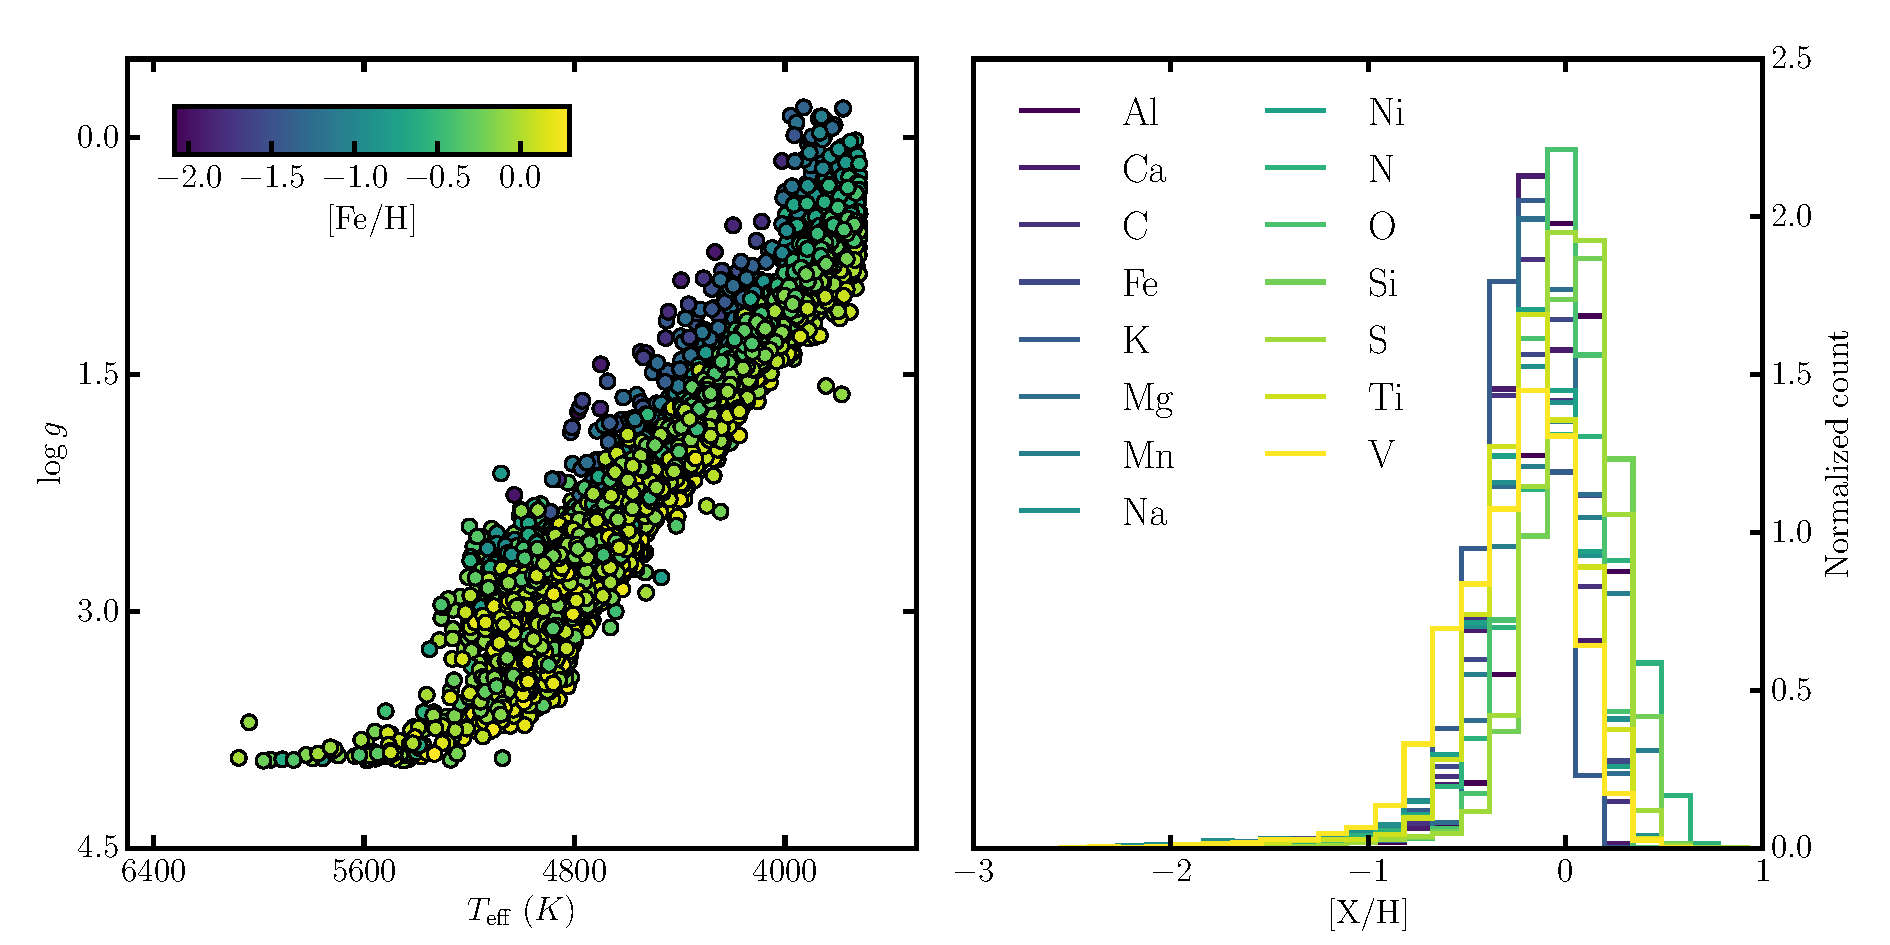
\includegraphics[width=\textwidth]{training_set_hrd.pdf}
\caption{A temperature-surface gravity diagram for all 12,681 stars in
the training set (left).  The distributions of abundances are shown for
all training set stars on the right.\label{fig:training_hrd}}
\end{figure}


\begin{figure}[p]
\caption{Choose two wavelengths (one continuum and one interesting)
  and plot some scatter plots of flux vs various parameters, and also
  cross-validation results for the
  hyper-parameters.\label{fig:onewavelength}}
\end{figure}

\begin{figure}[p]
\caption{Something about hyper-parameters and scatter as a function of
  wavelength.\label{fig:hyperpars}}
\end{figure}

\begin{figure}[p]
\caption{Something about first derivatives of the spectral expectation
  with respect to labels as a function of
  wavelength.\label{fig:derivatives}}
\end{figure}

\begin{figure}[p]
\caption{Show a few sample spectra and demonstrate that the quality of
  the model prediction is extremely good; better than
  \aspcap.\label{fig:correctness}}
\end{figure}

\begin{figure}[p]
\caption{Something showing that our results on the full unlabeled set
  make sense and seem correct!\label{fig:fulltest}}
\end{figure}


\begin{figure}[p]
\caption{Choose two elements that are interesting, and pull apart the
  differences between what we have and what \aspcap\ has for those
  elements.  We are better!\label{fig:elements}}
\end{figure}

\begin{figure}[p]
\caption{Something about the quality of results in the
  cross-validation as a function of the signal-to-noise of what we
  give in the test subset.\label{fig:snr}}
\end{figure}


\begin{figure}[p]
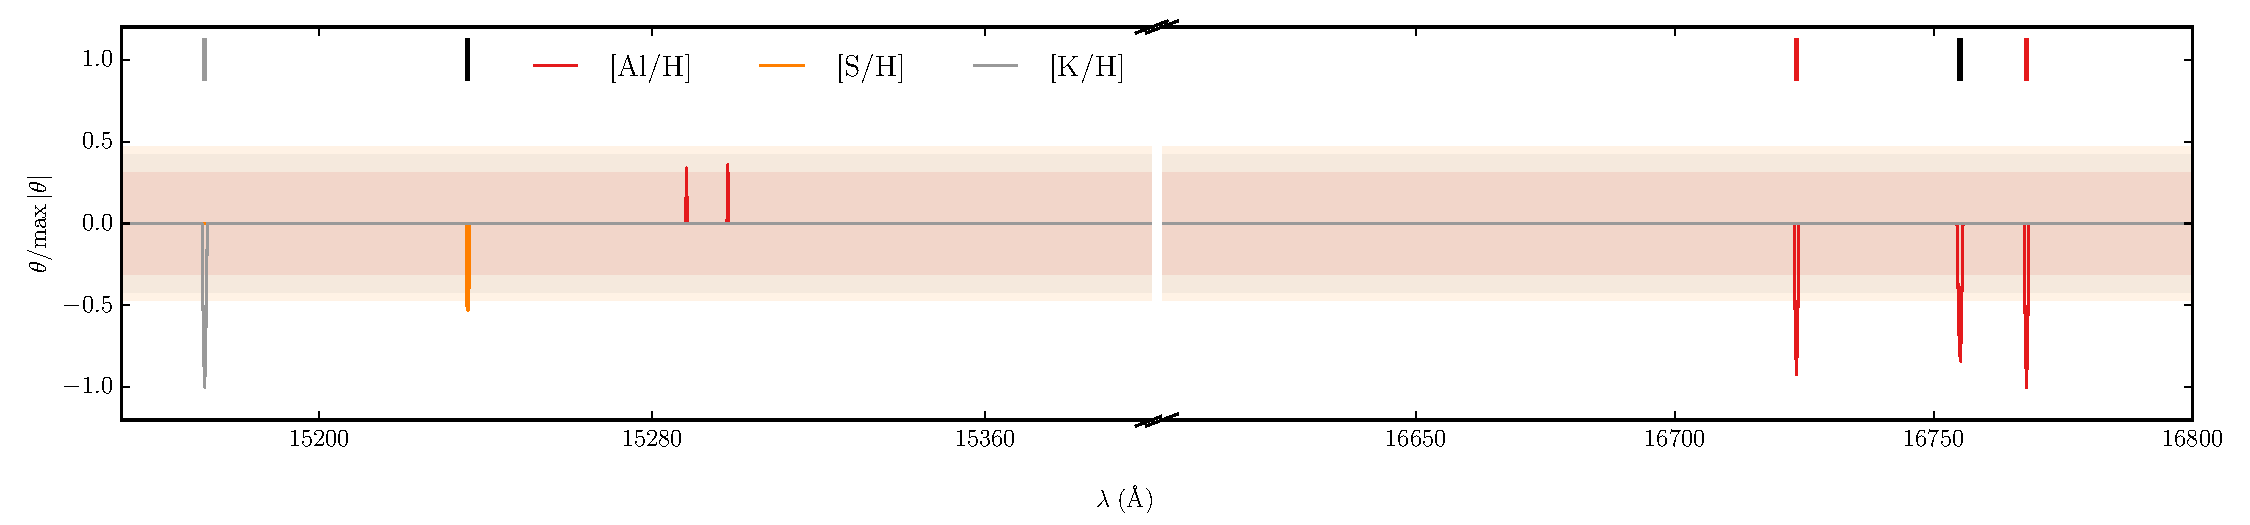
\includegraphics[width=\textwidth]{sparse-first-order-coefficients.pdf}
\caption{Normalized (to the maximum derivative value at any $\theta$) first-order derivatives for [Al/H], [S/H], and [K/H] from a regularized Cannon model with $\Lambda = 10^{3.5}$ and $f = 20$. For the sake of clarity, we have only shown $\theta$ values that exceed the shaded region. The top markings for K and Al correspond to the lines used by Smith et al. The black markers indicate 'Missing' or 'Unknown' lines in the APOGEE spectra according to Shetrone et al. Here we identify these elements from our model derivatives.  \label{fig:inferring-lines}}
\end{figure}

\begin{figure}[p]
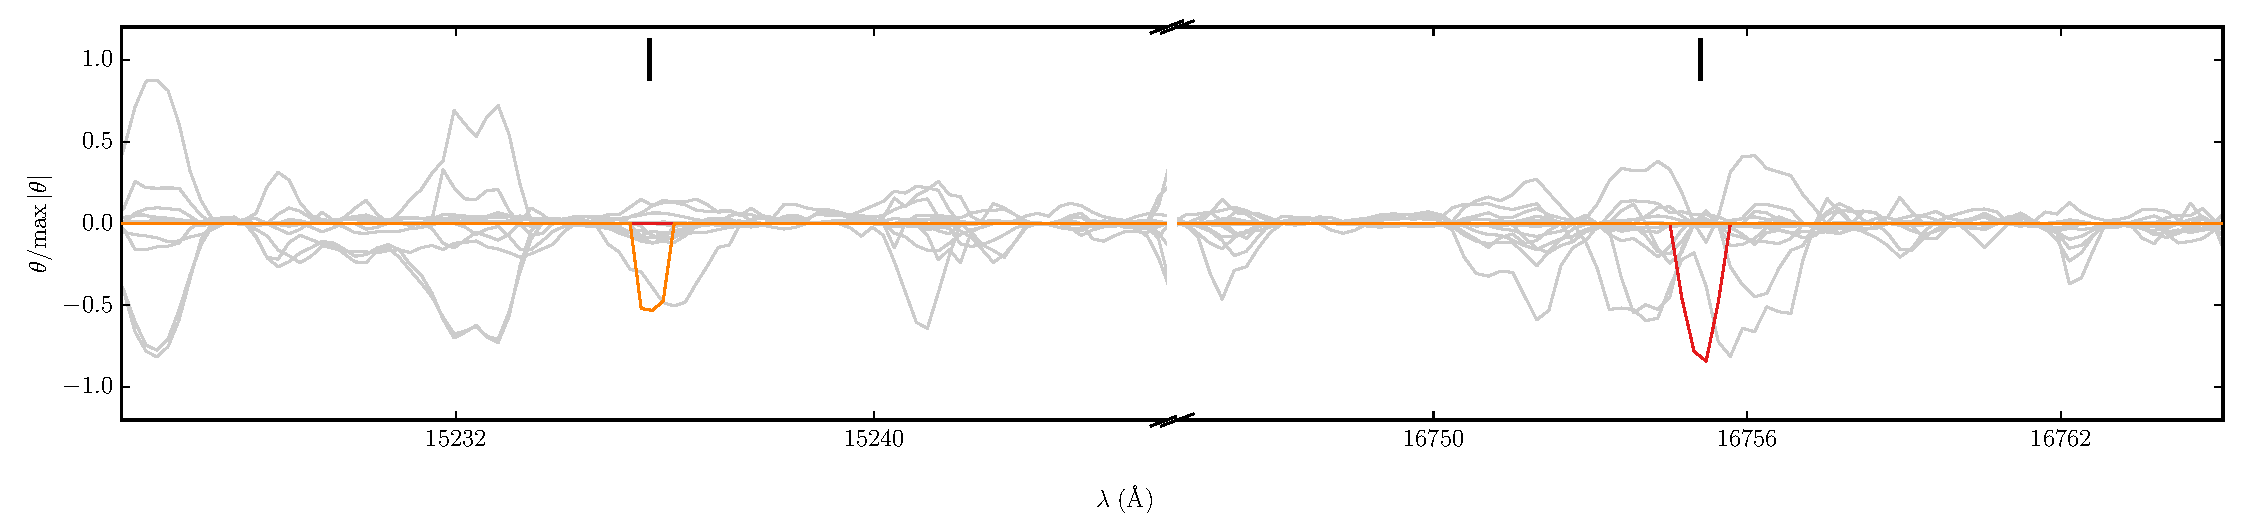
\includegraphics[width=\textwidth]{sparse-first-order-coefficients-zoom.pdf}
\caption{Zoom in of previous figure, showing the theta values for all elements. Al and S are highlighted and colored as per Figure \ref{fig:inferring-lines}.\label{fig:inferring-lines2}}
\end{figure}


\begin{figure}[p]
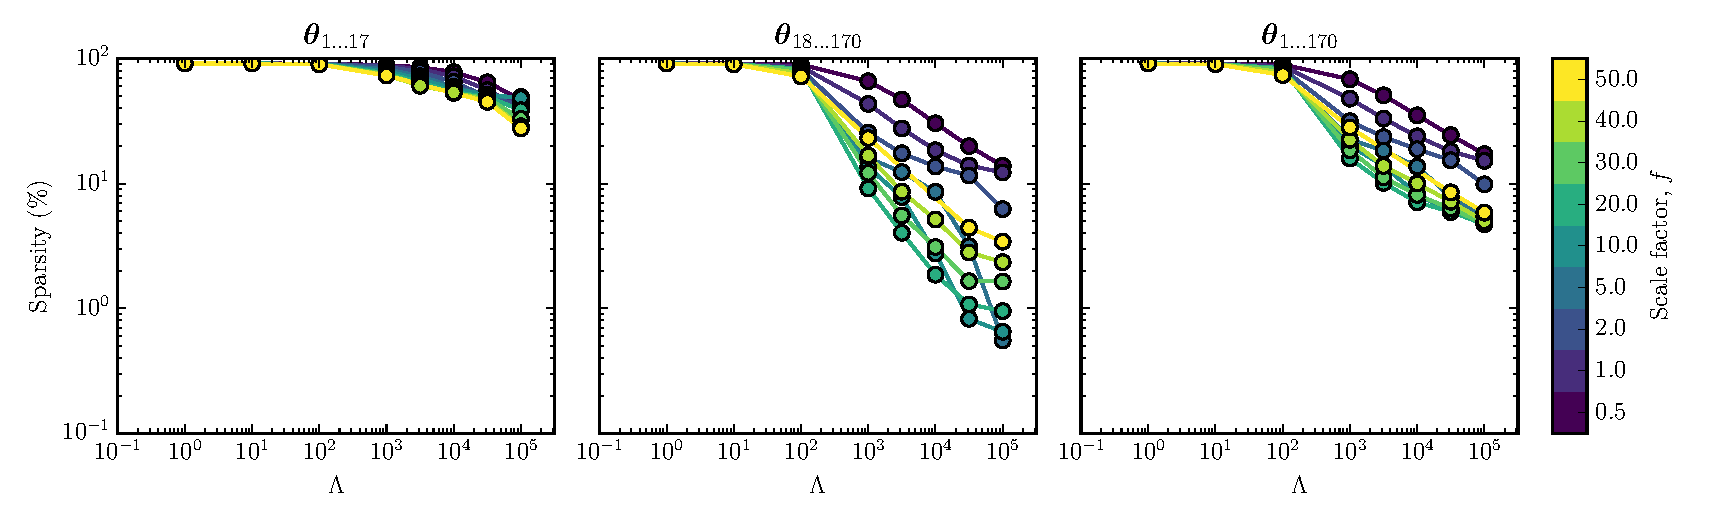
\includegraphics[width=\textwidth]{sparsity.pdf}
\caption{The fraction of non-zero coefficients (sparsity) of 17-label models with different scale factors $f$ and regularization terms $\Lambda$.  The sparsity of the first-order coefficients are shown in the left panel, the second-order coefficients (e.g., $\Teff^2$, $\Teff\cdot\logg$, or $[\rm{Al}/\rm{H}]\cdot[\rm{Mn}/\rm{H}]$) in the middle panel, and total sparsity (excluding the baseline spectrum coefficient $\theta_0$) in the right-hand panel.\label{fig:sparsity}}
\end{figure}


\begin{figure}[p]
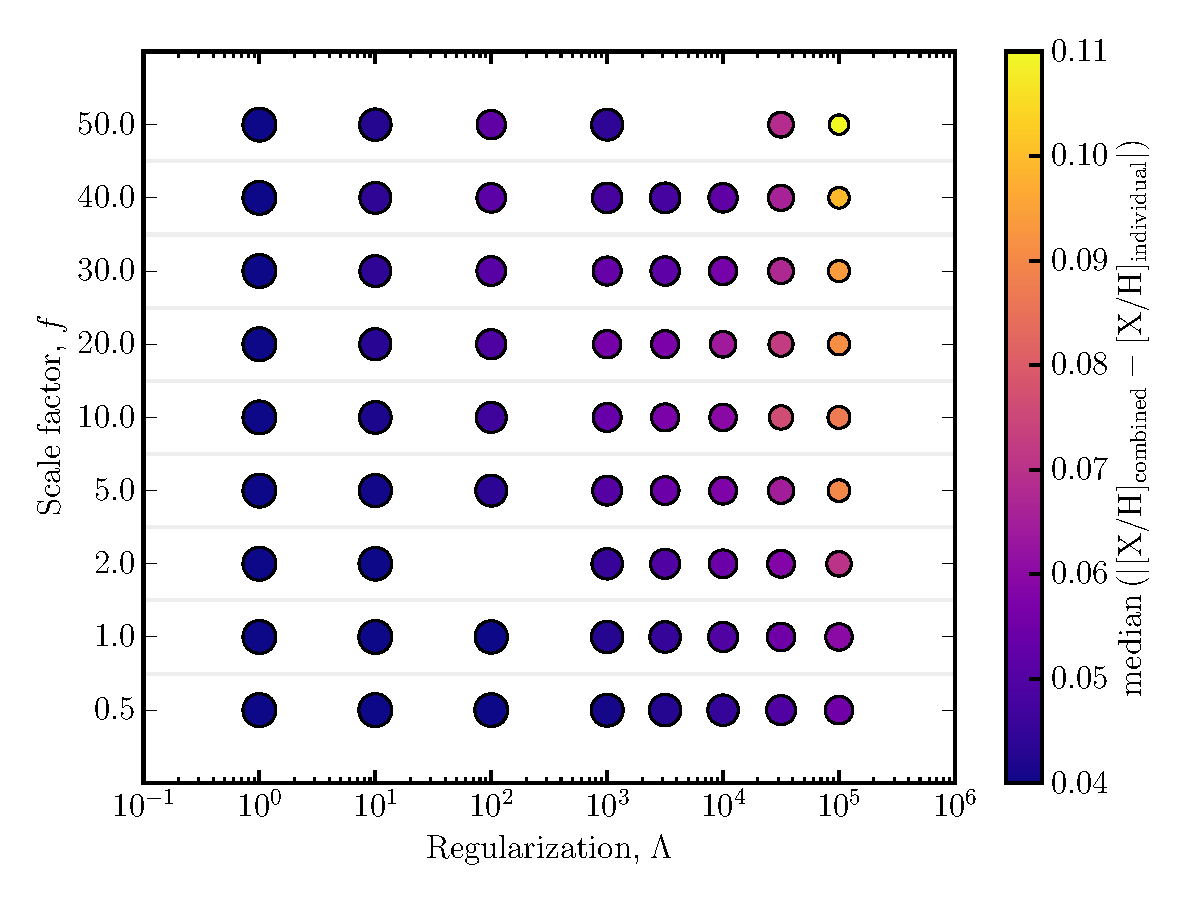
\includegraphics[width=\textwidth]{gs-mad-all-elements.pdf}
\caption{The median absolute abundance difference (over all abundance labels)
between that inferred from individual observations in the validation set, and
that inferred from the high $S/N$ combined spectrum.
\label{fig:gridsearch-mad-all-elements}}
\end{figure}




% These need rasterizing:
%\begin{figure}[p]
%\includegraphics[width=\textwidth]{high-alpha-seq-ASPCAP.pdf}
%\caption{A high [$\alpha$/Fe] sequence shown with \aspcap\ labels
%and coloured by the $S/N$ ratio.\label{fig:high-alpha-aspcap}}
%\end{figure}

%\begin{figure}[p]
%\includegraphics[width=\textwidth]{high-alpha-seq-TC.pdf}
%\caption{The same high [$\alpha$/Fe] stars shown in Figure
%\ref{fig:high-alpha-aspcap}, with abundances from \TheCannon.
%\label{fig:high-alpha-tc}}
%\end{figure}

\clearpage



\begin{figure}[p]
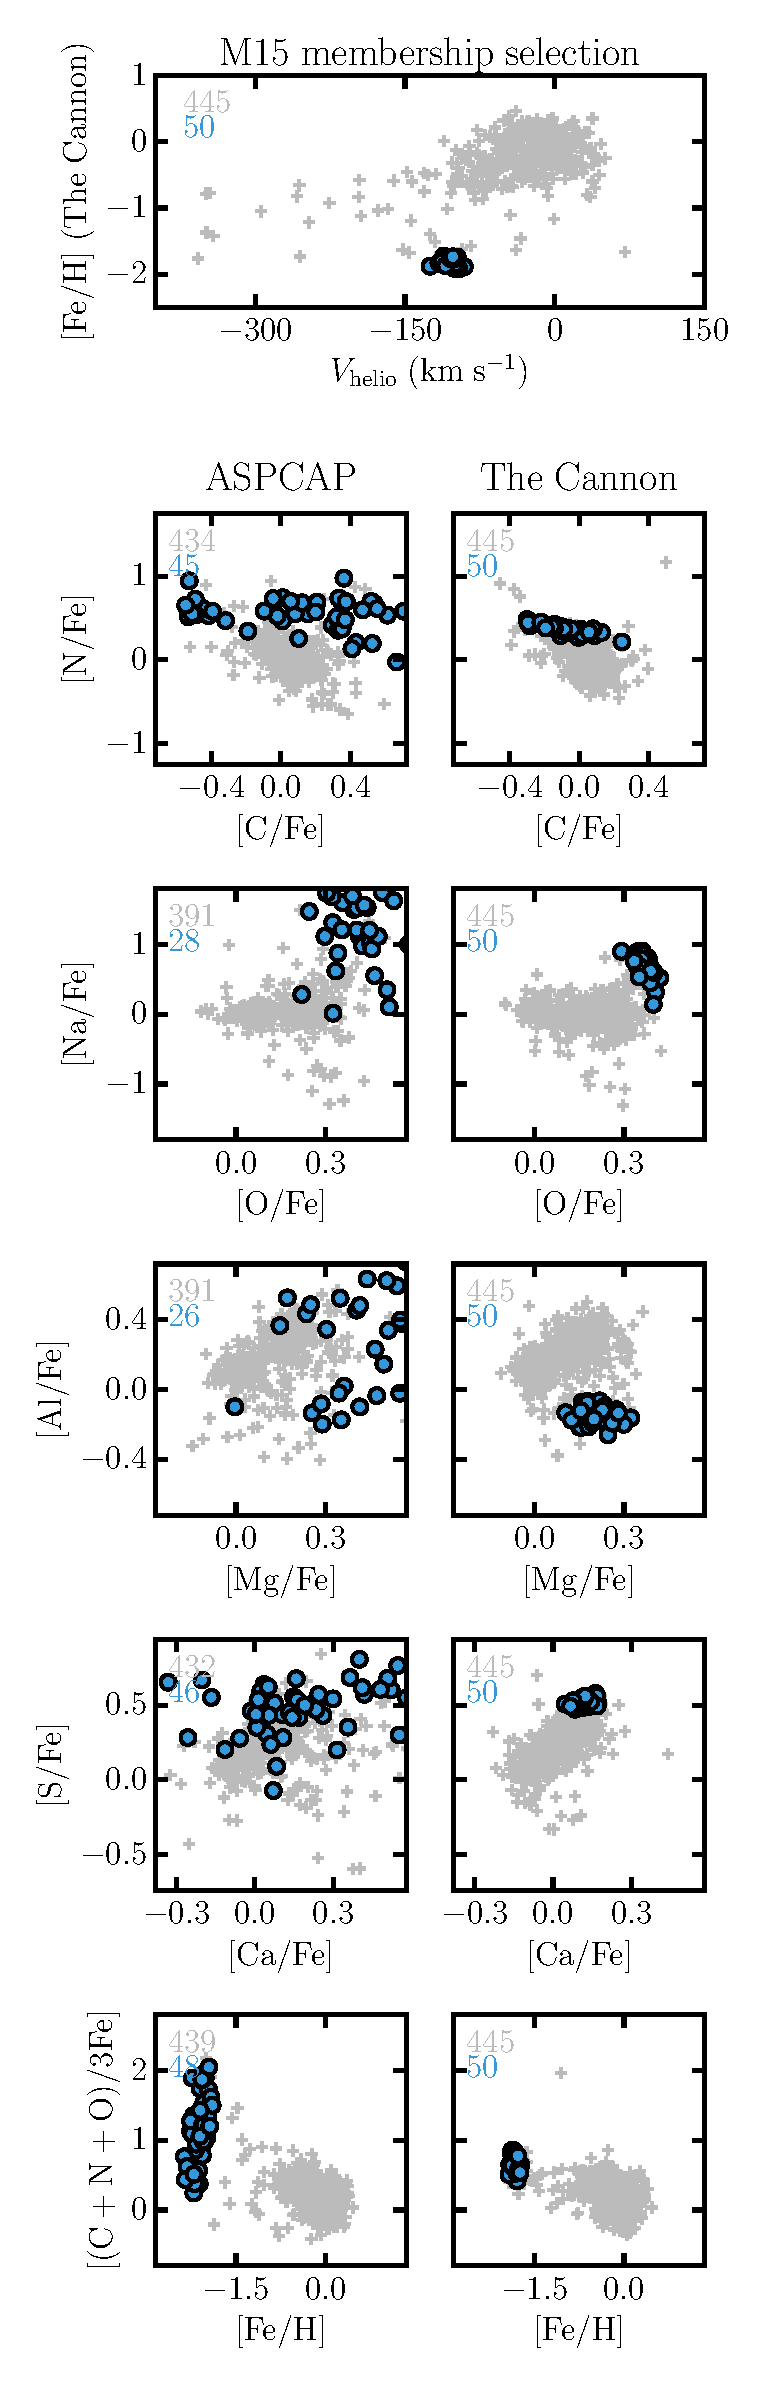
\includegraphics[width=0.40\textwidth]{M15_comparison.pdf}
\caption{Abundance labels from \aspcap\ and \TheCannon\ for candidate
members of the metal-poor globular cluster M~15 (NGC~7078).  The top panel
shows heliocentric velocity and metallicity, which we use to separate
bonafide cluster members (blue) from field stars (grey). The limits
in all abundance panels are set by the dynamic range of \TheCannon\ labels.
The number of stars within those limits (from \aspcap\ and \TheCannon)
are noted.\label{fig:m15-comparison}}
\end{figure}

\clearpage

\begin{figure}[p]
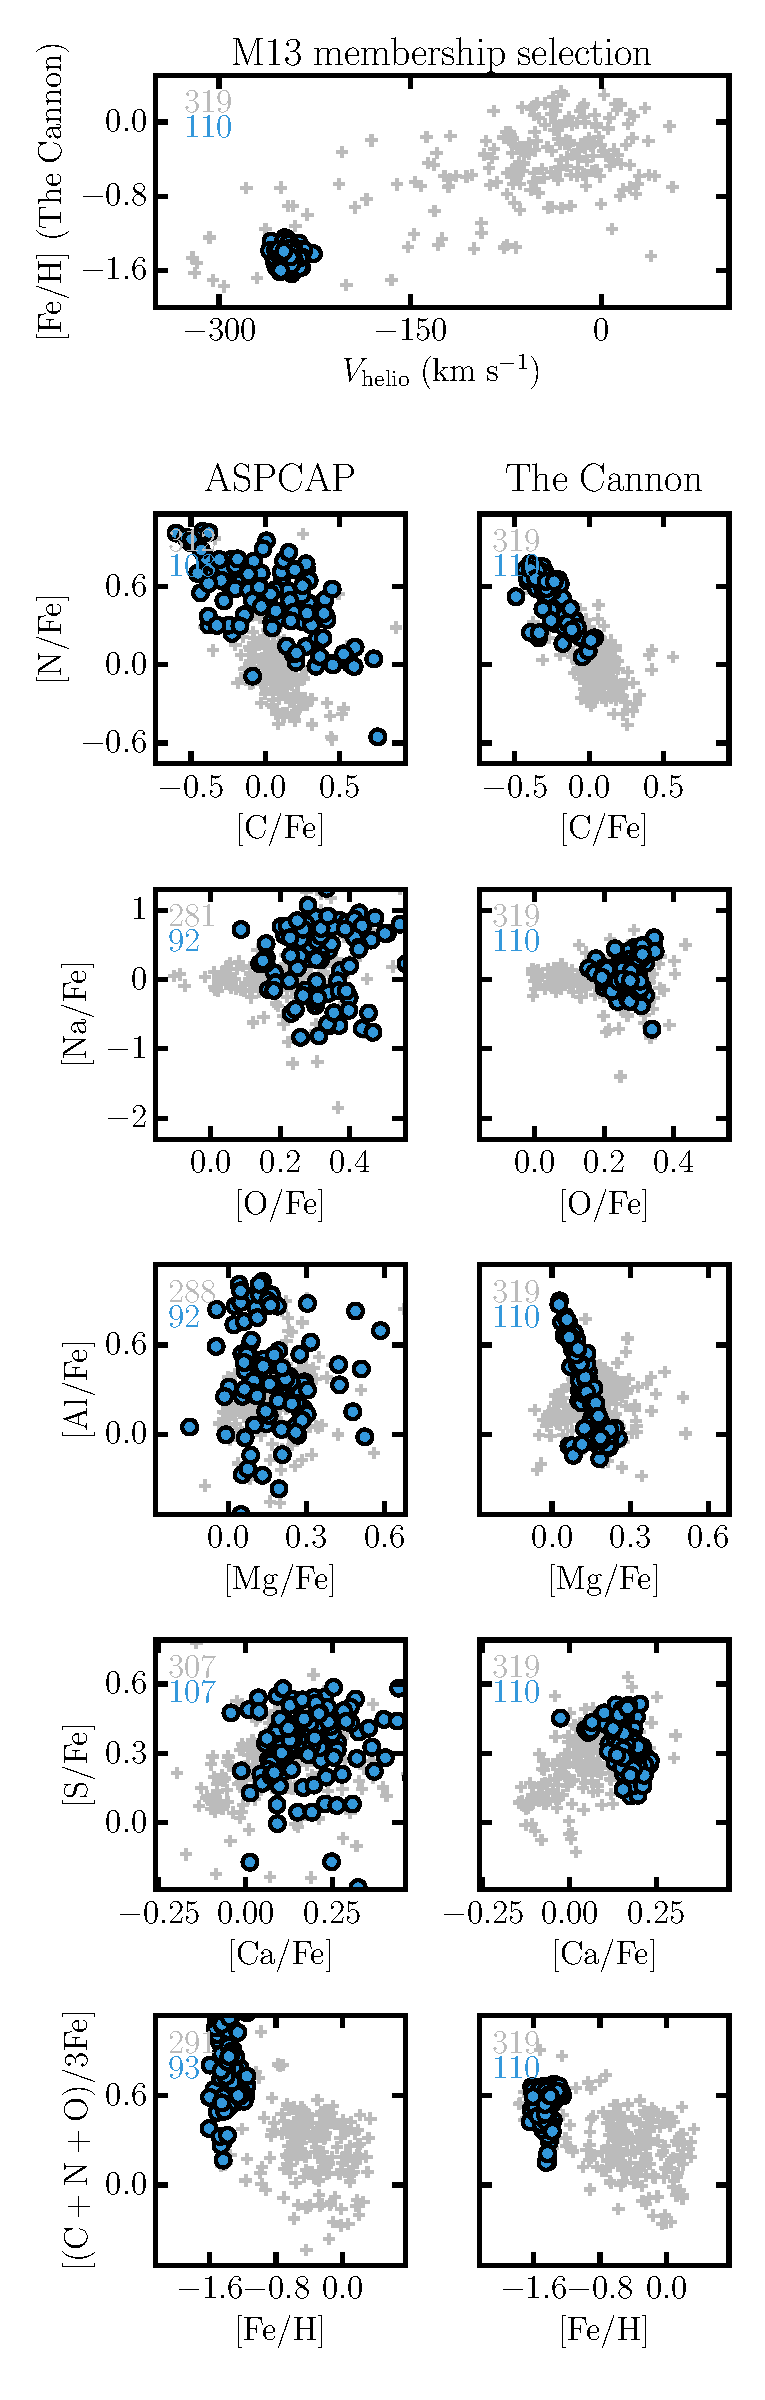
\includegraphics[width=0.4\textwidth]{M13_comparison.pdf}
\caption{Label comparison between \aspcap\ and \TheCannon\ for M~13.
Markings are the same as per Figure \ref{fig:m15-comparison}.
\label{fig:m13-comparison}}
\end{figure}

\clearpage

\begin{figure}[p]
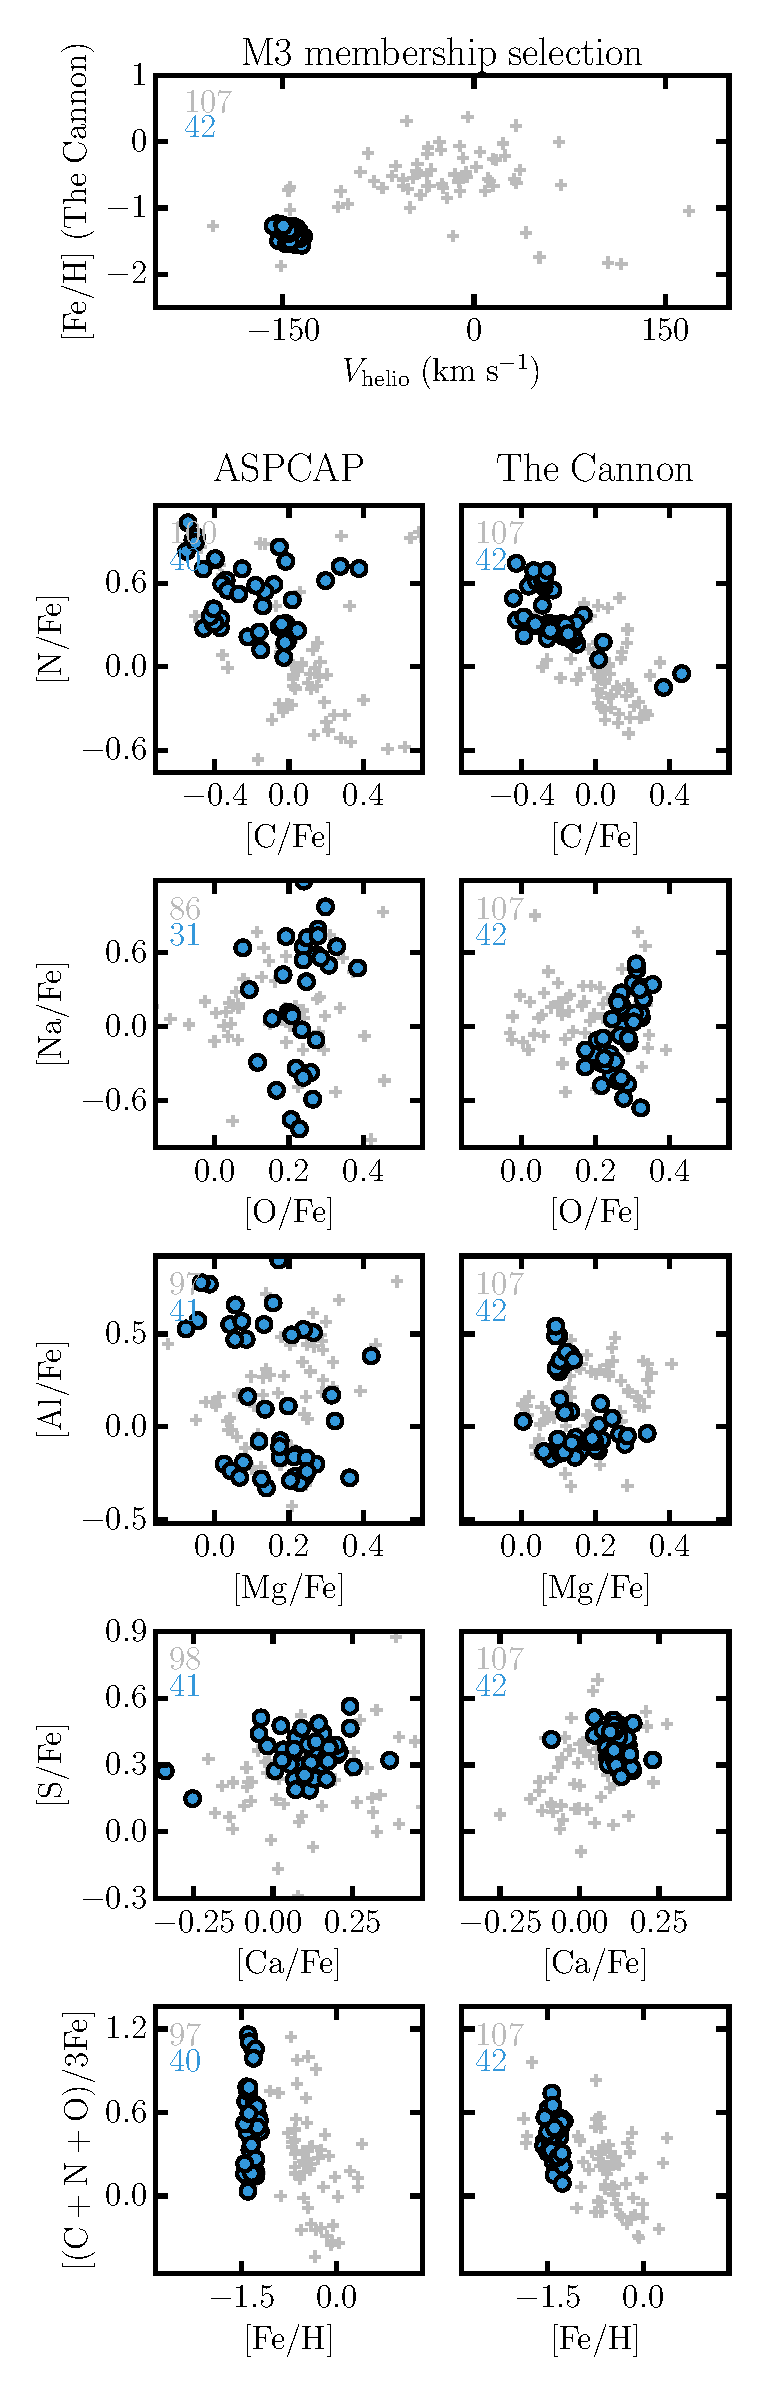
\includegraphics[width=0.4\textwidth]{M3_comparison.pdf}
\caption{Label comparison between \aspcap\ and \TheCannon\ for M~3.
Markings are the same as per Figure \ref{fig:m15-comparison}.
\label{fig:m3-comparison}}
\end{figure}

\clearpage

\begin{figure}[p]
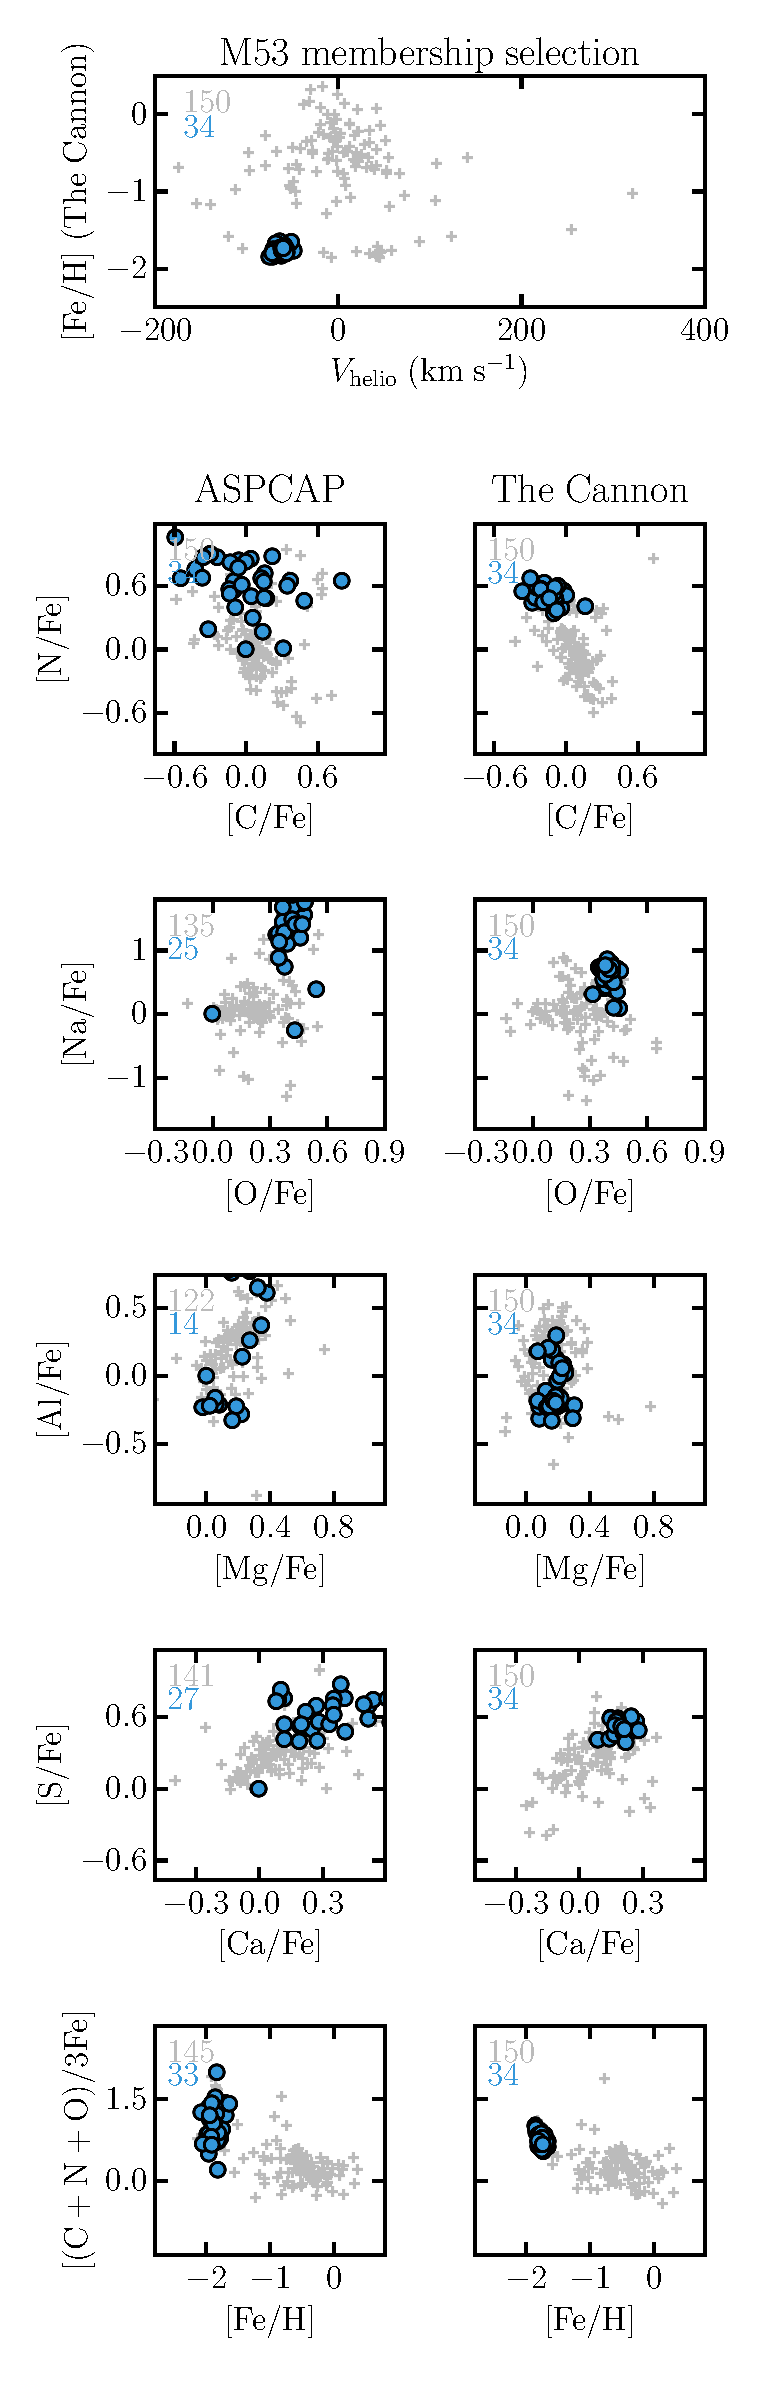
\includegraphics[width=0.4\textwidth]{M53_comparison.pdf}
\caption{Label comparison between \aspcap\ and \TheCannon\ for M~53.
Markings are the same as per Figure \ref{fig:m15-comparison}.
\label{fig:m53-comparison}}
\end{figure}

\clearpage

\begin{figure}[p]
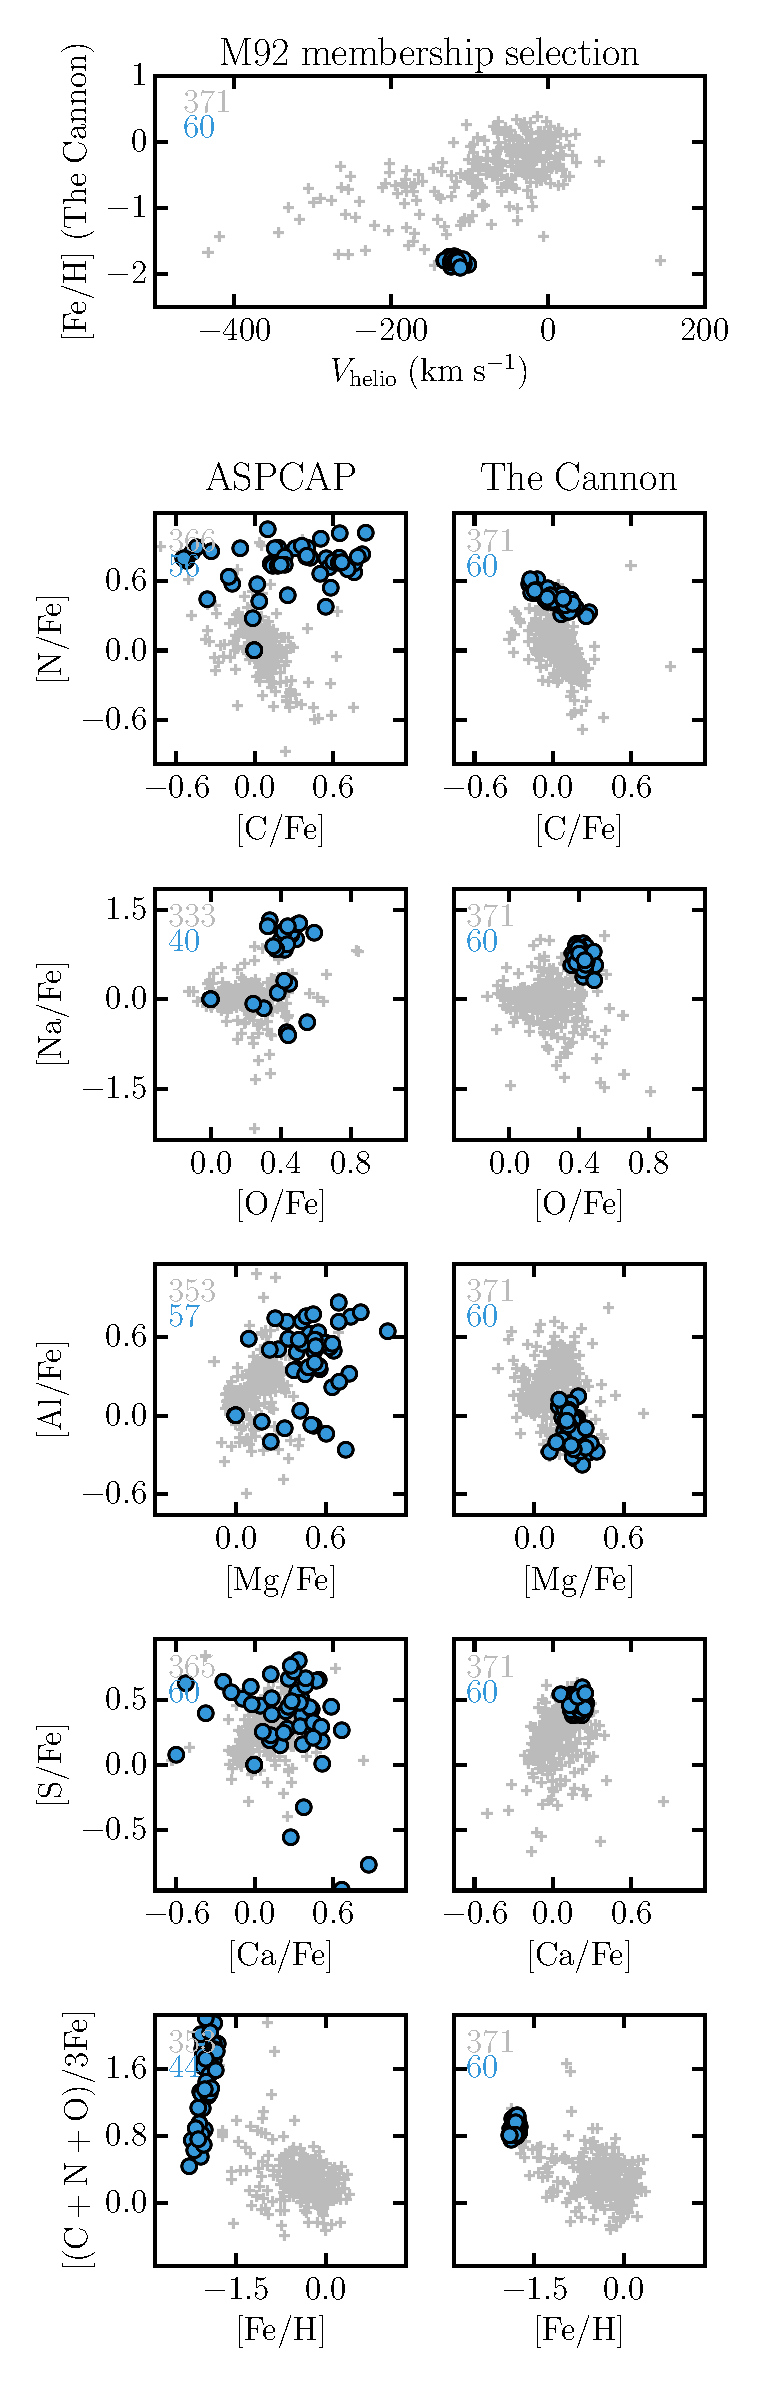
\includegraphics[width=0.4\textwidth]{M92_comparison.pdf}
\caption{Label comparison between \aspcap\ and \TheCannon\ for M~92.
Markings are the same as per Figure \ref{fig:m15-comparison}.
\label{fig:m92-comparison}}
\end{figure}


\end{document}


